\documentclass[final]{beamer}

% ====================
% Packages
% ====================

\usepackage[T1]{fontenc}
\usepackage{lmodern}
\usepackage[size=custom,width=120,height=90,scale=1]{beamerposter}
\usetheme{gemini}
\usecolortheme{cam}
\usepackage{graphicx}
\usepackage{booktabs}
\usepackage{tabularx}
\usepackage{tikz}
\usepackage{pgfplots}
\pgfplotsset{compat=1.14}
\usepackage{anyfontsize}
\usepackage{comment}
\usepackage{xcolor}
\usepackage[most]{tcolorbox}

\setbeamerfont{title}{size=\Huge}
\setbeamerfont{author}{size=\large}
\setbeamerfont{institute}{size=\normalsize}
\setbeamerfont{block title}{size=\Large}
\setbeamerfont{block body}{size=\large}
\setbeamerfont{caption}{size=\small}

\usepackage[skip=2pt]{caption}
\usepackage[backend=biber]{biblatex}
\addbibresource{ref.bib}

% --- Official blues ---
\definecolor{PrimaryBlue}{RGB}{29,79,145}        % #1D4F91
\definecolor{SecondaryBlue1}{RGB}{0,48,135}      % #003087
\definecolor{SecondaryBlue2}{RGB}{0,119,200}     % #0077C8
\definecolor{SecondaryBlue3}{RGB}{108,172,228}   % #6CACE4

% --- Neutral colors ---
\definecolor{Neutral1}{RGB}{34,34,34}       % #222222
\definecolor{Neutral2}{RGB}{83,86,90}       % #53565A
\definecolor{Neutral3}{RGB}{208,208,206}    % #D0D0CE
\definecolor{Neutral4}{RGB}{240,240,240}    % #F0F0F0

% --- Accent colors ---
\definecolor{Accent1}{RGB}{199,80,0}        % #C75000 — used for "confidence" everywhere

% Colour words that match the figures
\newcommand{\conf}[1]{\textcolor{Accent1}{\textbf{#1}}}
\newcommand{\struct}[1]{\textcolor{PrimaryBlue}{\textbf{#1}}}

% ====================
% Lengths
% ====================

% (N+1)*\sepwidth + N*\colwidth = \paperwidth
\newlength{\sepwidth}
\newlength{\colwidth}
\setlength{\sepwidth}{0.025\paperwidth}
\setlength{\colwidth}{0.3\paperwidth}

\newcommand{\separatorcolumn}{\begin{column}{\sepwidth}\end{column}}

% ====================
% Title
% ====================

\title{Think Before You Trust: \\ Where to Spend a Limited Verification Budget}
\author{Allison Li \and Xinyun (Alina) Du \and Christopher Lee}
\institute[shortinst]{Columbia University in the City of New York}

\footercontent{
  \href{https://github.com/backlight314/think-before-you-trust}{github.com/backlight314/think-before-you-trust} \hfill
  CSUREMM 2026 $\mid$ Supported by the Irving Institute for Cancer Dynamics, Dept.\ of Mathematics, Dept.\ of Statistics, Barnard SRI, and Jane Street \hfill
  al4936@columbia.edu, xd2364@columbia.edu, cl4371@columbia.edu
}

\begin{document}
\addtobeamertemplate{headline}{}
{
    \begin{tikzpicture}[remember picture,overlay]
      \node [anchor=north west, inner sep=3cm] at ([xshift=0.0cm,yshift=0.0cm]current page.north west)
      {\includegraphics[height=4.5cm]{logos/Columbia_University_Logo-white.png}};
    \end{tikzpicture}
    % QR code — check it is a permanent link to the repo
    \begin{tikzpicture}[remember picture,overlay]
      \node [anchor=north east, inner sep=3cm] at ([xshift=-6.0cm,yshift=0.8cm]current page.north east)
      {\includegraphics[height=7cm]{figures/qr-code.png}};
    \end{tikzpicture}
}

\begin{frame}[t]
\begin{columns}[t]
\separatorcolumn

% ================= COLUMN 1 — question & setup =================
\begin{column}{\colwidth}

  \begin{block}{Introduction}
    LLMs build a growing graph of dependent claims (lemmas and steps). One false claim can contaminate everything built on top of it, but verifying every step is too costly. Prior work focuses on \emph{how} to check a step; we ask \emph{which} steps to check when the budget only covers a few.

    The standard answer is to check the claims the model is least \conf{confident} about. But confidence is self-reported and often miscalibrated. The \struct{structure} of the reasoning graph --- which claims rest on which --- is a second signal that does not depend on calibration.
  \end{block}

  \begin{alertblock}{Research Questions}
    \begin{enumerate}
      \item Does the model's self-reported confidence help pick which claims to verify under a limited budget?
      \vspace{0.5em}
      \item Is there a structural signal that does as well, and stays useful when confidence is unreliable?
    \end{enumerate}
  \end{alertblock}

  \begin{block}{Setup}
    \begin{enumerate}
      \item \textbf{Generate.} A model expands a seed claim into a DAG of up to 50 dependent claims. Each claim has parents, a Python predicate, and a self-reported confidence $c(v)$.
      \item \textbf{Label.} A Python verifier checks every predicate over $n\in[-500,500]$. No LLM is involved in labelling.
      \item \textbf{Verify on a budget.} A strategy picks $k$ claims to check. A claim found false \emph{quarantines} all of its descendants, so one well-placed check can protect many claims.
    \end{enumerate}

    \textbf{Reliability} $=1-$ (false claims left undetected) $/$ (all claims).

    \begin{figure}
      \centering
      \begin{minipage}{0.49\linewidth}\centering
        \includegraphics[width=\linewidth]{figures/dag_snapshot.png}
      \end{minipage}\hfill
      \begin{minipage}{0.49\linewidth}\centering
        \includegraphics[width=\linewidth]{figures/llamaexample.png}
      \end{minipage}
      \caption{Left: simulated claim DAG (green $=$ true, red $=$ false, ringed $=$ verified). Right: a real dependency graph generated by Llama-3.1-8B.}
    \end{figure}
  \end{block}

  \begin{block}{Data}
    \begin{itemize}
      \item \textbf{Simulation:} random claim trees and DAGs. Error parameters from the PARC dataset: base error $\epsilon=0.176$, propagation $\rho=0.750$. Exact ceilings: dynamic programming (trees) and a Greedy-MC optimizer (DAGs).
      \item \textbf{Real LLMs:} 8 models (Claude Haiku 4.5, Gemini, DeepSeek, Qwen-80B, GPT-OSS-120B, GPT-OSS-20B, Llama-70B, Llama-8B) $\times$ 45 runs over 15 number-theory seed claims $=$ \textbf{14{,}600+} machine-checked claims.
    \end{itemize}
  \end{block}

\end{column}

\separatorcolumn

% ================= COLUMN 2 — strategies & main result =================
\begin{column}{\colwidth}

  \begin{block}{Verification Strategies}
    \begin{table}\centering
      \caption{Each strategy ranks claims and checks the top $k$.}
      \vspace{-0.5em}
      \renewcommand{\arraystretch}{1.1}
      \begin{tabular}{@{}lll@{}}
        \toprule
        \textbf{Strategy} & \textbf{Signal} & \textbf{Scores a claim by} \\
        \midrule
        Random            & none                 & baseline \\
        Uncertainty-first & \conf{confidence}    & lowest $c(v)$ \\
        Dependency-aware  & \struct{structure}   & descendant count $|\mathrm{desc}(v)|$ \\
        Betweenness       & \struct{structure}   & paths running through $v$ \\
        Expected damage   & both                 & $(1-c(v))\cdot(|\mathrm{desc}(v)|+1)$ \\
        Oracle            & true labels          & ceiling, not deployable \\
        \bottomrule
      \end{tabular}
    \end{table}
  \end{block}

  \begin{alertblock}{Main Finding}
    \centering
    On real reasoning graphs from 8 LLMs at a 10\% budget, \\[0.3em]
    \struct{structure beats random on 8 / 8 models}, \\
    \conf{confidence falls below random on 5 / 8}. \\[0.3em]
    On the six models with $>40\%$ error, structure adds \textbf{+0.18} reliability over confidence.
  \end{alertblock}

  \begin{block}{Result 1: Real LLMs}
    \begin{figure}\centering
      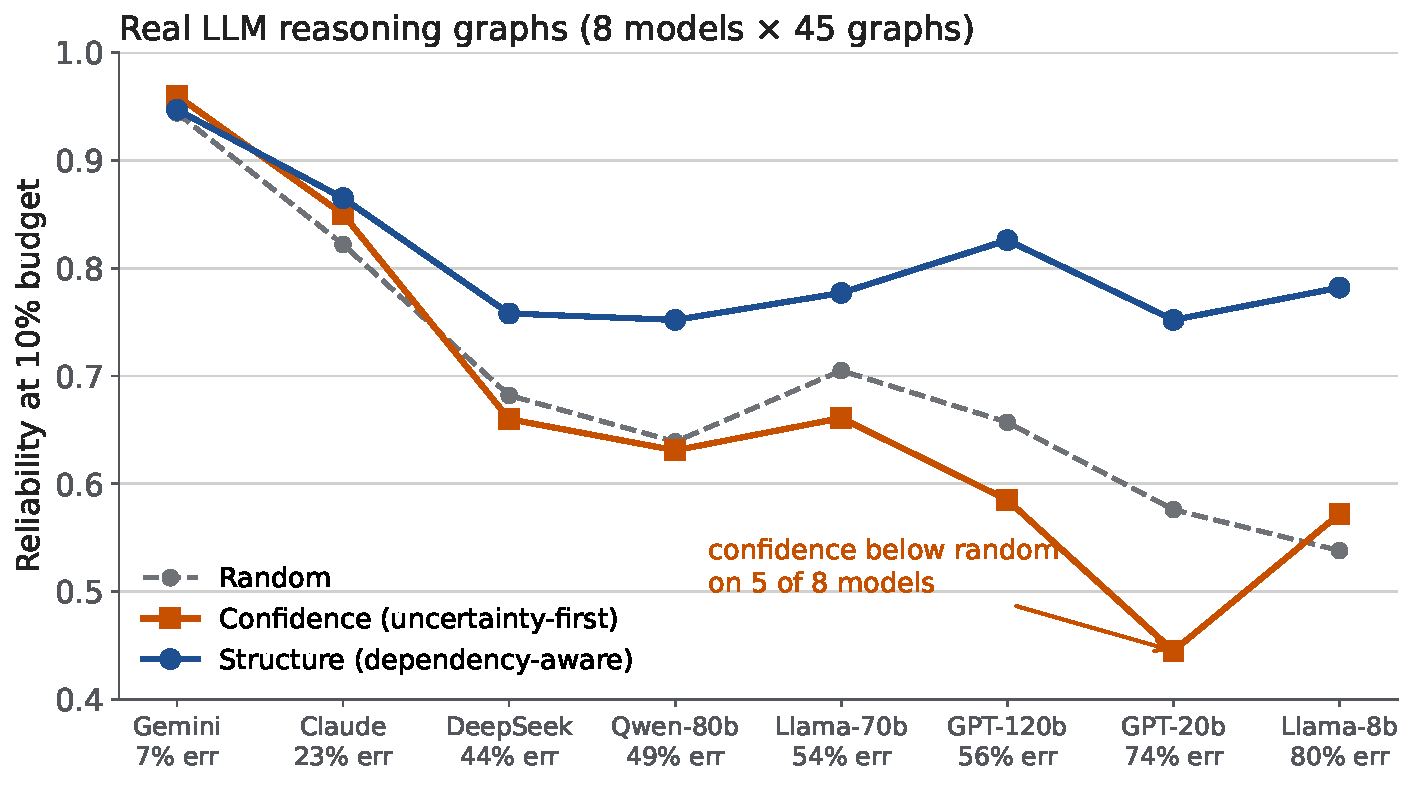
\includegraphics[width=\linewidth]{figures/fig_real_llm.pdf}
      \caption{Reliability at a 10\% budget, models ordered by error rate. When models make few errors the two signals tie; as errors rise, confidence-based checking collapses while structure stays at 0.75--0.95.}
    \end{figure}

    \begin{table}\centering\small
      \caption{All strategies at a 10\% budget (mean reliability, 45 graphs per model). Bold $=$ best non-oracle strategy.}
      \vspace{-0.5em}
      \setlength{\tabcolsep}{11pt}
      \begin{tabular}{lrrrrrr}
        \toprule
        \textbf{Model} & \textbf{Random} & \textbf{Uncert.} & \textbf{Dep-aware} & \textbf{Exp.\ dmg} & \textbf{Betw.} & \textbf{Oracle} \\
        \midrule
        Claude       & $0.822$ & $0.850$ & $0.865$ & $\mathbf{0.877}$ & $0.823$ & $0.962$ \\
        Gemini       & $0.944$ & $0.960$ & $0.947$ & $\mathbf{0.963}$ & $0.944$ & $0.998$ \\
        DeepSeek     & $0.682$ & $0.660$ & $0.758$ & $\mathbf{0.760}$ & $0.714$ & $0.897$ \\
        GPT-OSS-120B & $0.657$ & $0.585$ & $\mathbf{0.826}$ & $0.785$ & $0.671$ & $0.968$ \\
        GPT-OSS-20B  & $0.576$ & $0.445$ & $\mathbf{0.752}$ & $0.693$ & $0.554$ & $0.909$ \\
        Llama-70B    & $0.705$ & $0.661$ & $0.777$ & $\mathbf{0.804}$ & $0.681$ & $0.931$ \\
        Llama-8B     & $0.538$ & $0.572$ & $\mathbf{0.782}$ & $0.698$ & $0.529$ & $0.880$ \\
        Qwen-80B     & $0.639$ & $0.631$ & $\mathbf{0.752}$ & $0.731$ & $0.682$ & $0.893$ \\
        \bottomrule
      \end{tabular}
    \end{table}
  \end{block}

\end{column}

\separatorcolumn

% ================= COLUMN 3 — supporting results & conclusion =================
\begin{column}{\colwidth}

  \begin{block}{Result 2: Simulation}
    On synthetic DAGs, a cheap structural signal matches an expensive optimizer.
    \begin{figure}\centering
      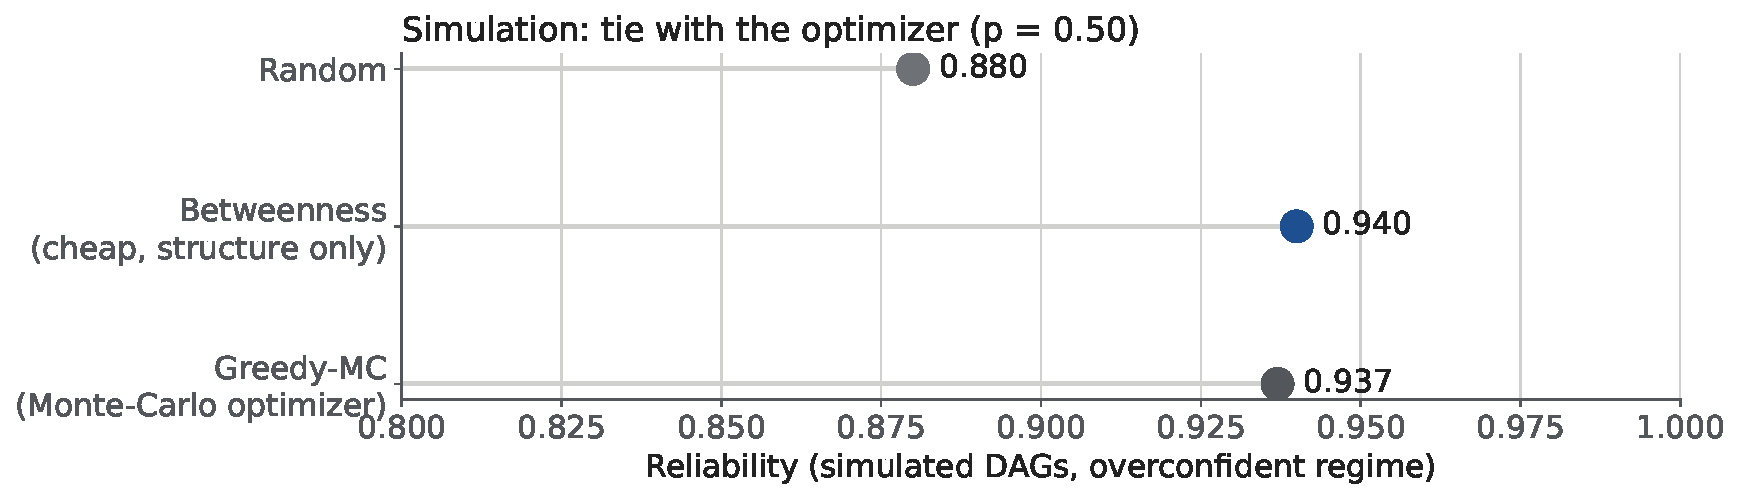
\includegraphics[width=\linewidth]{figures/fig_simulation.pdf}
      \caption{Simulated DAGs, overconfident regime. Betweenness centrality (no confidence used) ties the Monte-Carlo greedy optimizer (0.940 vs.\ 0.937, $p=0.50$). On real graphs betweenness is close to random (Table 2): descendant count is the structural signal that transfers.}
    \end{figure}
  \end{block}

  \begin{block}{Result 3: Corrupting Confidence}
    Confidence is controlled by the model. On a small set of real traces we corrupted \emph{only} the confidences, keeping the reasoning and labels fixed.
    \begin{figure}\centering
      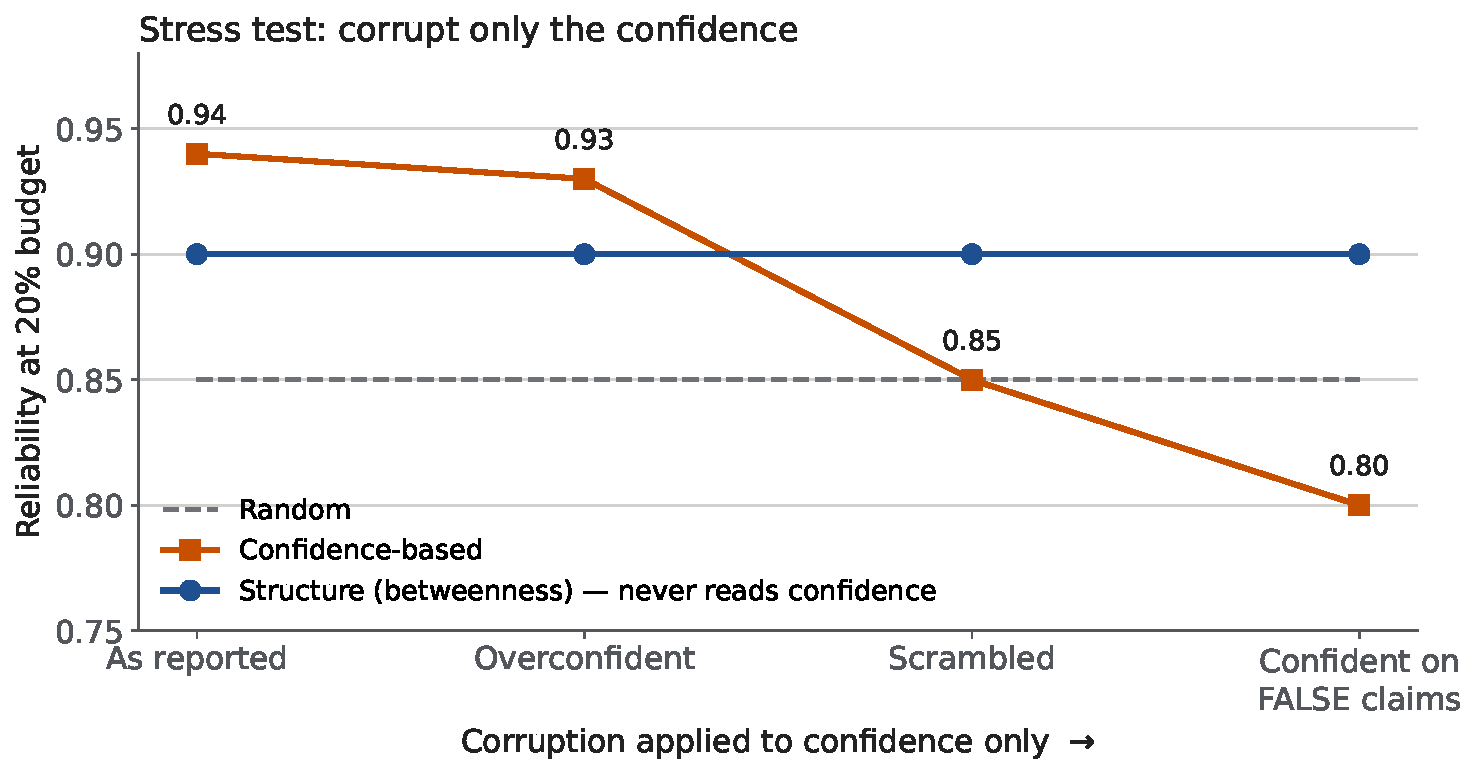
\includegraphics[width=\linewidth]{figures/fig_robustness.pdf}
      \caption{When confidence is honest, it leads slightly. When the model is confident on its false claims, confidence-based checking falls below random (paired bootstrap gap $+0.102$, $p<0.001$). Structure is unaffected because it never reads confidence. Stress test on 7 real traces.}
    \end{figure}

    \begin{table}\centering\small
      \caption{Calibration. Every model is confident on its false claims, and the true/false gap is thin (inverted for Llama-8B).}
      \vspace{-0.5em}
      \setlength{\tabcolsep}{14pt}
      \begin{tabular}{lrrrrr}
        \toprule
        \textbf{Model} & \textbf{Claims} & \textbf{Err\%} & \textbf{conf$|$T} & \textbf{conf$|$F} & \textbf{Gap} \\
        \midrule
        Claude       & $2148$ & $23\%$ & $0.91$ & $0.81$ & $0.10$ \\
        Gemini       & $2200$ &  $7\%$ & $1.00$ & $0.95$ & $0.05$ \\
        DeepSeek     & $1450$ & $44\%$ & $0.92$ & $0.69$ & $0.23$ \\
        GPT-OSS-120B & $2161$ & $56\%$ & $0.90$ & $0.78$ & $0.12$ \\
        GPT-OSS-20B  & $2117$ & $74\%$ & $0.84$ & $0.66$ & $0.18$ \\
        Llama-70B    & $1461$ & $54\%$ & $0.83$ & $0.70$ & $0.13$ \\
        Llama-8B     & $1472$ & $80\%$ & $0.81$ & $0.82$ & $-0.01$ \\
        Qwen-80B     & $1620$ & $49\%$ & $0.97$ & $0.93$ & $0.04$ \\
        \bottomrule
      \end{tabular}
    \end{table}
  \end{block}

  \begin{block}{Conclusion}
    \begin{itemize}
      \item \conf{Confidence} is a real but thin signal: the true/false gap ranges from $-0.01$ to $0.23$, and it is the best way to land checks directly on false claims.
      \item \struct{Structure} is the better guide for \emph{containing} errors: descendant count beats random on all 8 models and beats confidence on 7 of 8.
      \item Structure is \emph{harder} to fake, not impossible: an LLM-judge audit finds 8--39\% spurious dependency edges.
      \item \textbf{Next:} verification inside agentic loops that expand, check, and backtrack as they reason.
    \end{itemize}
  \end{block}

\end{column}

\separatorcolumn
\end{columns}
\end{frame}
\end{document}
